\subsection{An intuitive explanation of the DFT -1/2 method}
This method aims to expand the half-occupation technique \cite{PhysRevB.5.844}\cite{SLATER19721}, formalized by Janak’s theorem, to crystals using modern exchange-correlation approaches \cite{PhysRevB.23.5048} \cite{PhysRevLett.77.3865}.

The Slater half-occupation scheme has already proven to be quite efficient for calculating atomic ionization energy values close to the experimental ones. However, this technique cannot be applied blindly to extended systems like crystals, since the crystal is described by means of Bloch waves, and removing the population of just one Bloch state would have no consequences \cite{PhysRevB.78.125116}. Moreover, removing the population of one Bloch State and setting periodic conditions would result in an infinitely charged system.

Thus, the proposed solution is to apply the Slater procedure to crystalline energy bands. The intuition for this application comes from the fact that the energy bands of a crystal are formed by the overlap of atomic orbitals, mainly by those that constitute the outermost layers. This relationship can be quantified by the projection of the wave function in a given orbital, Figure \ref{bs_BN} shows the character for each atom in the band structure of the h-BN, the bigger the blue dots, the stronger the character. Thereby, considering this existing relationship, self-energy corrections performed in atoms could propagate and shift the energy of the bands, resulting in a band gap correction.

\begin{figure}[!ht]
        \centering
        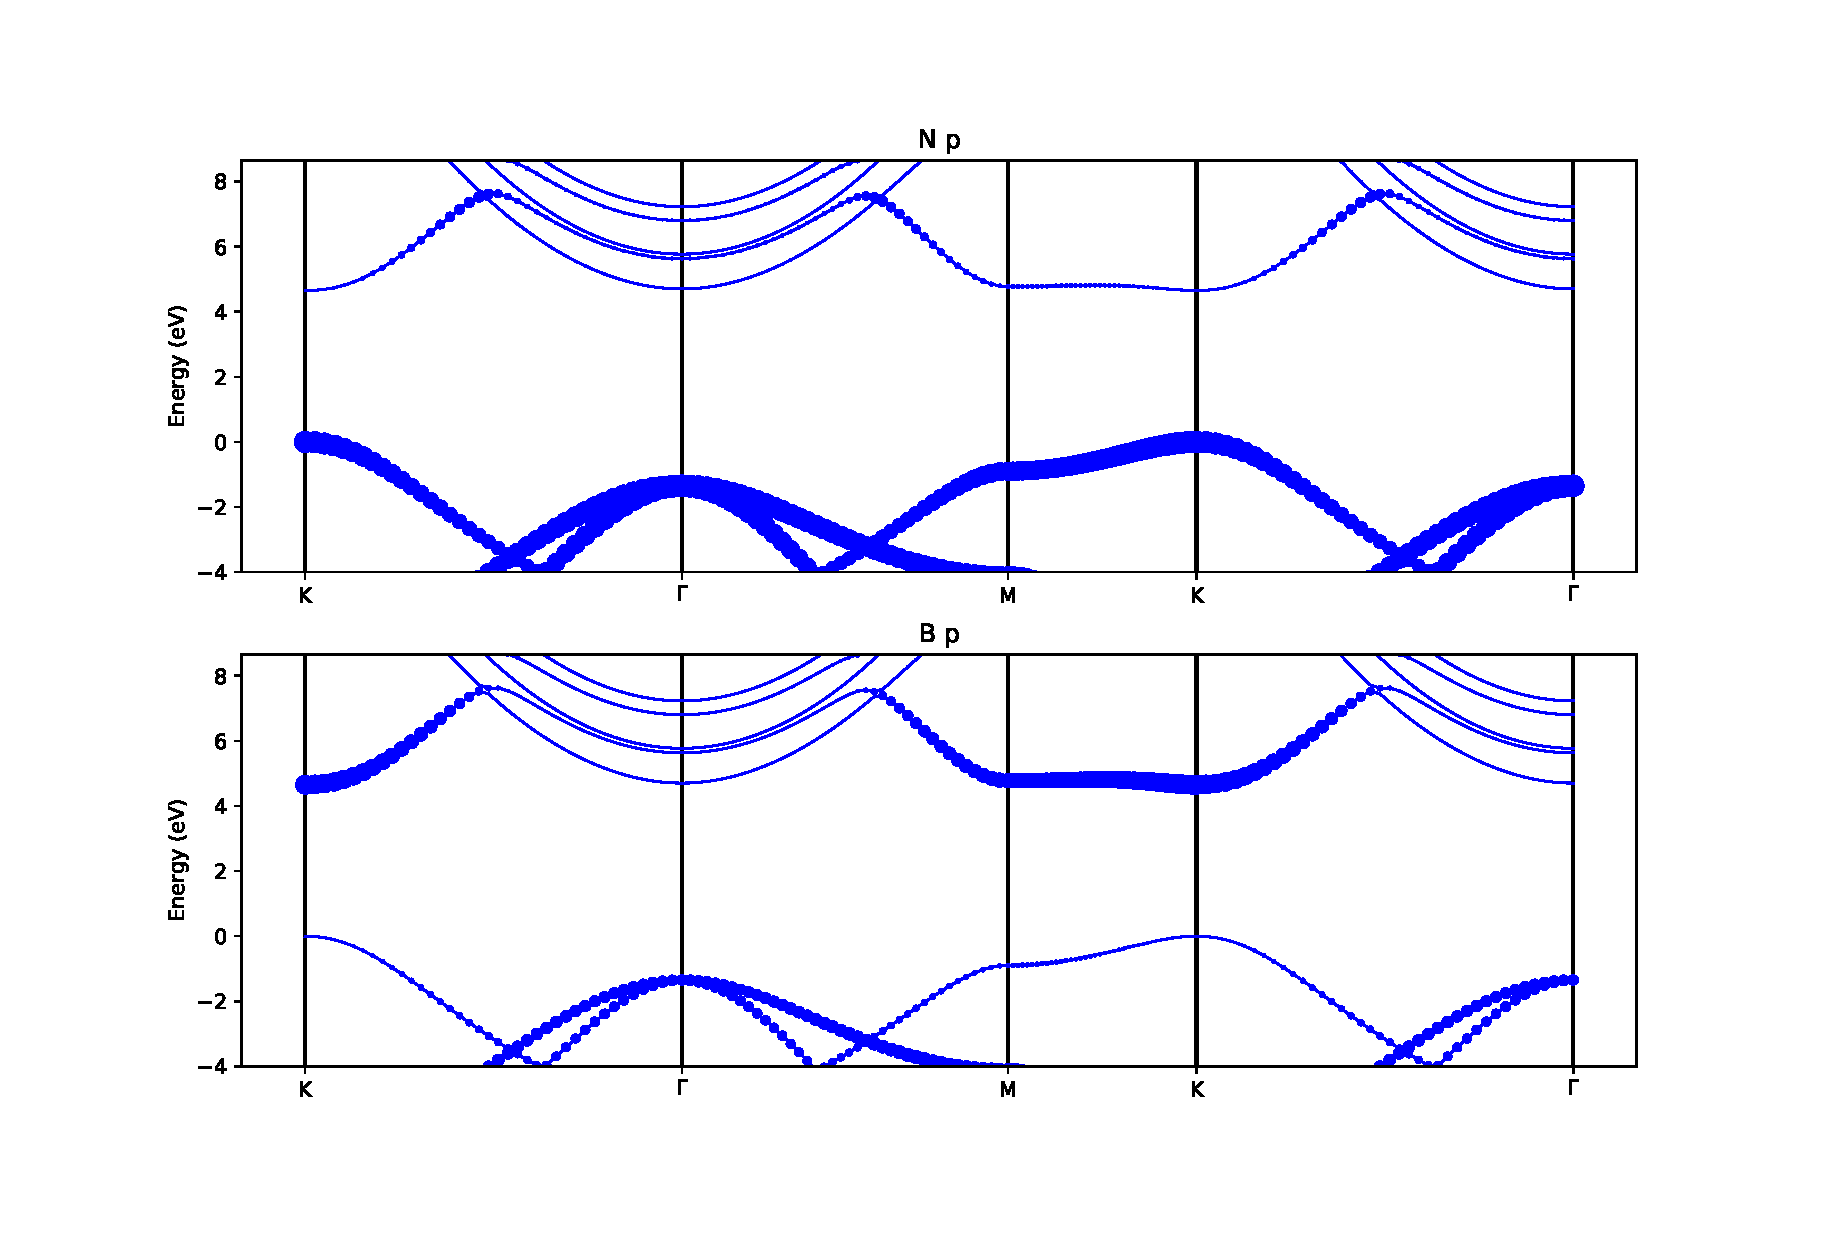
\includegraphics[width=15cm,height=12cm]{images/bands.eps}
        \caption{$p$ character for each atom in the h-BN band structure. The bigger the blue dots, the stronger the character.}
        \label{bs_BN}
\end{figure}

\subsection{How to perform potential correction in crystals}

In this section, calculations were developed using some approximations in order to demonstrate
intuitively how the potential correction in crystals is made. To access the rigorous demonstration, consult the references \cite{PhysRevB.78.125116} \cite{doi:10.1063/1.3624562}. 

Following the Slater half occupation procedure for atoms, a change in charge density is required
to obtain the potential for semi-occupation and perform self-consistent calculations using the Kohn-Sham equation.

Although in extended systems like crystals, a change in charge density in a unit cell would result in an infinitely charged system, which would lead to a 
divergence in the Kohn-Sham calculations. Furthermore, it would also be irrelevant to be able to modify only a finite amount of electrons in the crystal, since
the charge would become irrelevant to the infinite amount of electrons present in the system. To bypass this problem, it is necessary to find a new way
to derive the semi-occupied potential.

Firstly, one has to define the system that corresponds to the semi-occupied potential for a solid. For an atom containing
$N$ electrons in its ground state, the semi-occupied potential is defined as the potential of the atom with $N-\frac{1}{2}$ electrons. Similarly, we should consider that the semi-occupied potential of a solid would be the potential generated by a solid with $M-\frac{1}{2}$ electrons per primitive cell, where $M$ is the number of electrons
of the unit cell in the ground state, as shown in Figure \ref{semi-solid}.

\begin{figure}[!ht]
        \centering
        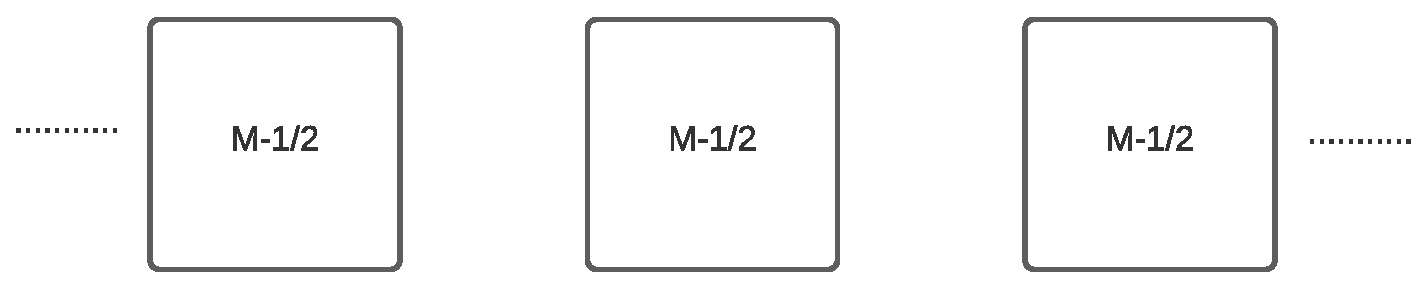
\includegraphics[width=10cm,height=2cm]{images/semi-solid.eps}
        \caption{Scheme representing the unit cells of a solid that would generate the potential semi-occupied.}
        \label{semi-solid}
\end{figure}
So, to outline the solution, suppose one have $N$ independent charge distributions, where the $mth$ is given by:

\begin{equation}
    \rho_{m}(\vec{\mathbf{R}}) = (1+f_{m})n_{m}(\vec{\mathbf{R}}) 
\end{equation}

\begin{equation}
n_{m}(\vec{\mathbf{R}}) = -q \cdot \eta_{m}    
\end{equation}

\begin{equation}
 \int \eta_{m}(\vec{\mathbf{R}})d\vec{\mathbf{R}} = 1   
\end{equation}


Where $\rho$ represents the density of the distribution $m$, $q$ represents the charge of the electron, $\eta$ a normalized function in space, and $f$ represents an occupancy factor that varies continuously from 0 (occupied) to -1 (unoccupied).

Considering the charge density represented above, one can find the Coulomb potentials for each distribution
by the Poison equation:

\begin{equation}
   \nabla^{2}V_{m}(\vec{\mathbf{R}}) = \frac{q\rho_{m}(\vec{\mathbf{R}})}{\epsilon_{0}}
\end{equation}

Now, suppose another situation where one only alternates the occupation of the $\alpha$ level, and the same charge distribution remains. In this scenario, the $mth$ potential is given by:

\begin{equation}
\nabla^{2}V_{m}{'}(\vec{\mathbf{R}}) = \frac{q\rho_{m}{'}(\vec{\mathbf{R}})}{\epsilon_{0}}  
\end{equation}

\begin{equation}
f_{i}=f_{i}{'}, i \neq \alpha 
\end{equation}

\begin{equation}
f_{\alpha} \neq f_{\alpha}{'} 
\end{equation}

Thus, one wants to calculate the potential for all distributions, which is obtained by adding
of the potential of all distributions, as shown in the equations below.

\begin{equation}
\nabla^{2}V(\vec{\mathbf{R}}) = \frac{q\sum_{m=1}^{N}\rho_{m}}{\epsilon_{0}}   \\
\end{equation}

\begin{equation}
\nabla^{2}V{'}(\vec{\mathbf{R}}) = \frac{q\sum_{m=1}^{N}\rho_{m}{'}}{\epsilon_{0}}  
\end{equation}
   
Subtracting these two equations:

\begin{equation}
\nabla^{2}(V(\vec{\mathbf{R}})-V{'}(\vec{\mathbf{R}})) = \frac{q(f_{\alpha}-f_{\alpha}{'})n_{\alpha}(\vec{\mathbf{R}})}{\epsilon_{0}}    
\end{equation}
   

Using the above equation for the specific case of $f_{\alpha} = 0$ and $f_{\alpha}{'} = -1/2$, the following equation is obtained:

\begin{equation}
\nabla^{2}(V(\vec{\mathbf{R}})-V{'}(\vec{\mathbf{R}})) = \frac{qn_{\alpha}(\vec{r})}{2\epsilon_{0}}\Rightarrow V{'}(\vec{\mathbf{R}}) = V(\vec{\mathbf{R}}) - V_{\alpha}^{f_{\alpha}=-1/2}    
\end{equation}
   
Hence, using the equation above, one can calculate the potential semi-occupied from other potentials, which discards the need to modify the charge density. For a crystal, the equation is written as follows:
\subsection{Unraveling Band Gap Underestimation in DFT}
The discrepancy in the accuracy of the band gap calculation using DFT arises from the need to incorporate a discontinuity in the derivative of energy in relation to the number of particles in the system. However, this discontinuity is not evidenced in the currently studied approximations for the exchange-correlation functional, such as the local gradient (LDA) and generalized gradient (GGA) approximations. Consequently, the DFT underestimates the band gap value by around $40\%$ \cite{PhysRevLett.51.1884}. In table  this discrepancy can be clearly observed in a few semiconductors.
\subsection{Local density approximation (LDA)}
Local Density Approximation (LDA) \cite{PhysRev.140.A1133} is a popular non-empirical method in Density Functional Theory (DFT) for calculating the exchange-correlation functional of a system. The LDA seeks to introduce the uniform electron gas as the reference system and assumes that the exchange-correlation energy of the original system at a specific point $\mathbf{R}_{0}$ can be approximated by the exchange-correlation energy of the reference system as long as it has the same electronic density at the point $\mathbf{R}_{0}$.

One may mathematically write the LDA functional as:

\begin{equation}
E_{xc}^{LDA}[\eta(\mathbf{R})] = \int \epsilon_{xc}^{hom}(\eta(\mathbf{R})) d\mathbf{R},
\end{equation}

where $\epsilon_{xc}^{hom}(\eta(\mathbf{R}))$ is the exchange-correlation energy of the reference system consisting of a uniform gas of electrons with density $\eta(\mathbf{R})$.

As a result of using a reference system such as the homogeneous electron gas, the LDA has some limitations, such as the inability to capture the non-locality of the exchange-correlation potential and the self-interaction error. However, this method manages to produce surprising results, such as errors from $1\%$ to $5\%$ in molecular energies and errors from $1\%$ to $2\%$ in \cite{DFTCoursera} lattice constants.


\subsection{Generalized gradient approximation (GGA)}
In order to solve the aforementioned problems, a widely used class of approximations is the generalized gradient approximation (GGA), which takes into account not only the local density of electrons but also their gradient.

One may mathematically write the GGA functional as:

\begin{equation}
E_{xc}^{GGA}[\eta (\mathbf{R})] = \int \epsilon_{xc}^{hom}(\eta(\mathbf{R}))F_{xc}(\eta^ {\sigma}(\mathbf{R}), \nabla \eta^{\sigma}(\mathbf{R})) d\mathbf{R},
\end{equation}

where $\eta(\mathbf{R})$ is the electron density at position $\mathbf{R}$, $\nabla\eta(\mathbf{R})$ is its gradient, $\epsilon_ {xc}^{hom}$ is the exchange-correlation energy considering the uniform electron gas reference system and $F_{xc}$ is an improvement factor that depends on the local spin density $\eta^{\sigma}(\mathbf{R})$ and its gradient $\nabla\eta^{\sigma}(\mathbf{R})$.

A commonly used GGA functional is the Perdew-Burke-Ernzerhof (PBE) functional \cite{PhysRevLett.77.3865}. This functional has shown good results for a wide variety of systems.

\subsection{Functional and Functional derivatives}
To address the concept of functional, one must first address the concept of functions. A function is a rule that maps a number $x$ to another number $f(x)$. Similarly, a functional is a rule that maps a function $f(x)$ to a number $F[f]$. For instance, the expected value of energy in quantum mechanics is a functional that links the function $\psi$ to the number $\langle \psi | \hat{H} | \psi \rangle$ \cite{parr1994density}.

Another important concept to be understood is functional derivatives. Functional derivatives are a mathematical expression that relates the change in a functional $F[f]$ with respect to an infinitesimal change $\epsilon \cdot \alpha (x)$ in the function $f$. Thus, it can be defined that if the first derivative of the functional referring to $\epsilon$ exists, it can be written as:

\begin{equation}
    \frac{d F[f + \epsilon \cdot \alpha (x)]}{d \epsilon} \bigg|_{\epsilon =0} = \int \frac{\delta F[f]}{\delta f(x)} \alpha(x) dx
\end{equation}

The functional derivative is the expression $\frac{\delta F[f]}{\delta f(x)}$.

To understand the topics discussed below, it is important to know three classifications applied to functionals: Local, semi-local, and non-local. Each of these terms will be explained below:

\begin{itemize}
\item Local functionals: A local functional is a functional that depends only on the function at a single point in space.

\item Semilocal functionals: A semi-local functional is a functional that depends on the function and its derivatives evaluated at a single point in space.

\item Nonlocal functionals: A non-local functional is a functional that depends on a function and its derivatives evaluated at distant points in space.
\end{itemize}


\subsection{The CUT parameter} 
As observed for several 3D and 2D materials \cite{PhysRevB.97.045426}, one may observe that a $CUT$ parameter has a strong dependence on the considered element where the half occupation is applied, as shown in Figure \ref{cut-element-2d} for two-dimensional materials, which is consistent with the environment neglect and the isolated atom approximation for the self-energy potential. The significant differences between CUT parameters for one element in distinct materials are explained by the difference between bond lengths in the studied materials. In general, materials with smaller first-neighbor lengths exhibit smaller cutoff parameters. A linear relation between the $CUT$ parameter and the bond lengths (d) is observed for several classes of 2D materials \cite{PhysRevB.97.045426} and 3D materials \cite{PhysRevB.78.125116}.

\begin{figure}[!ht]
        \centering
        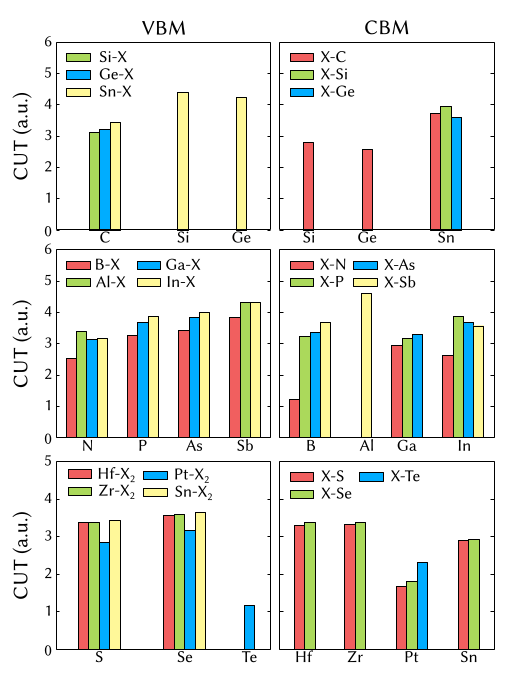
\includegraphics[width=13cm,height=15cm]{images/cut_element_2d.png}
        \caption{Cutoff parameter comparison for a selected set of 2D
    materials. The cutoff parameters of the VBM (CBM) states on the
   anions (cations) are represented on the left (right)\cite{PhysRevB.97.045426} .}
        \label{cut-element-2d}
\end{figure}
%.. figure:: images/cut_element_2d.png
%   :align: center
%   :width: 500

%   Fig 4. [12]_.
